\begin{figure}[ht]
    \tikzset{every picture/.style={line width=0.75pt}} %set default line width to 0.75pt
    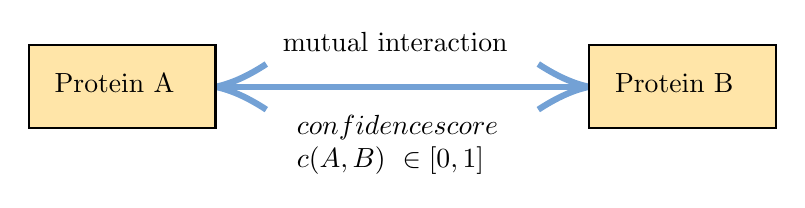
\begin{tikzpicture}[x=0.75pt,y=0.75pt,yscale=-1,xscale=1]
        %uncomment if require: \path (0,136); %set diagram left start at 0, and has height of 136

        %Straight Lines [id:da5202946805882411]
        \draw [color={rgb, 255:red, 115; green, 161; blue, 213 }  ,draw opacity=1 ][fill={rgb, 255:red, 0; green, 0; blue, 0 }  ,fill opacity=1 ][line width=2.25]    (114,40) -- (286,40) ;
        \draw [shift={(290,40)}, rotate = 180] [color={rgb, 255:red, 115; green, 161; blue, 213 }  ,draw opacity=1 ][line width=2.25]    (24.48,-10.98) .. controls (15.57,-5.15) and (7.41,-1.49) .. (0,0) .. controls (7.41,1.49) and (15.57,5.15) .. (24.48,10.98)   ;
        \draw [shift={(110,40)}, rotate = 0] [color={rgb, 255:red, 115; green, 161; blue, 213 }  ,draw opacity=1 ][line width=2.25]    (24.48,-10.98) .. controls (15.57,-5.15) and (7.41,-1.49) .. (0,0) .. controls (7.41,1.49) and (15.57,5.15) .. (24.48,10.98)   ;
        %Shape: Rectangle [id:dp8315683426496481]
        \draw  [fill={rgb, 255:red, 255; green, 229; blue, 168 }  ,fill opacity=1 ] (20,20) -- (110,20) -- (110,60) -- (20,60) -- cycle ;
        %Shape: Rectangle [id:dp6227729030936355]
        \draw  [fill={rgb, 255:red, 255; green, 229; blue, 168 }  ,fill opacity=1 ] (290,20) -- (380,20) -- (380,60) -- (290,60) -- cycle ;

        % Text Node
        \draw (31,32) node [anchor=north west][inner sep=0.75pt]   [align=left] {Protein A};
        % Text Node
        \draw (301,32) node [anchor=north west][inner sep=0.75pt]   [align=left] {Protein B};
        % Text Node
        \draw (141,12) node [anchor=north west][inner sep=0.75pt]   [align=left] {mutual interaction};
        % Text Node
        \draw (141,50.4) node [anchor=north west][inner sep=0.75pt]    {$ \begin{array}{l}
                                                                              \text{confidence score}\\
                                                                              c( A,B) \ \in [ 0,1]
        \end{array}$};
    \end{tikzpicture}
    \caption{Schematic of an interaction between two proteins}
\end{figure}
